\chapter{Scalaz} % Main chapter title

\label{Chapter1} % Change X to a consecutive number; for referencing this chapter elsewhere, use \ref{ChapterX}

Scalaz\footnote{\url{https://github.com/scalaz/scalaz}} è una libreria open source per la programmazione funzionale, che mette a disposizione un grande numero di strutture dati puramente funzionali create per integrare quelle della Scala Standard Library. In Scalaz sono presenti diversi nuovi elementi, definiti principalmente sotto forma di type class, ma anche delle estensioni per le strutture dati standard.

Scalaz rappresenta un progetto molto ampio, tanto che la prima release risale al 2010 e l'ultima a pochi giorni fa e che si sono sviluppati diversi progetti a partire da esso (come ad esempio Scalaz IO, poi trasformatosi nello standalone ZIO, una libreria per la programmazione asincrona e concorrente). Perciò sarà approfondita soltanto una parte delle strutture dati disponibili in Scalaz, con un duplice obiettivo: fornire una panoramica significativa della libreria ed introdurre gli elementi che saranno utilizzati per l'implementazione del caso d'uso presentato in questo elaborato.

%----------------------------------------------------------------------------------------
%	SECTION 1
%----------------------------------------------------------------------------------------

\section{Sezione 1}

\newpage

\subsection{Semigroup e Monoid}

In matematica, un semigruppo è definito come una \textit{struttura dati algebrica costituita da un insieme di elementi munito di un'operazione binaria associativa} (funzione che associa a due elementi di un tipo un terzo elemento dello stesso tipo). Analizzando questo concetto nell'ambito della programmazione, un semigruppo può essere costituito, ad esempio, da un insieme di stringhe e dall'operazione di concatenazione oppure da un insieme di interi e da un'operazione quale addizione, moltiplicazione o elevamento a potenza.

Scalaz mette a disposizione il trait Semigroup[S], e ogni sua implementazione (type class) rappresenta un semigruppo. Esso soddisferà due regole:

\begin{itemize}
\item \textit{Chiusura}: $\forall$ a, b $\in$ S, append(a, b) $\in$ S. È garantita dal type system.
\item \textit{Associatività}: $\forall$ a, b, c $\in$ S, append(append(a,b),c) = append(a,append(b,c)).
\end{itemize}

Inoltre Scalaz definisce l'operatore \textit{mappend} e il suo alias simbolico |+| che, tramite il meccanismo di method injection (e quindi usando gli impliciti), possono essere richiamati su un oggetto per il cui tipo è stata definita un'istanza di Semigroup e restituiscono la ``combinazione'' dei due oggetti.

\lstinputlisting[caption=Definizione di Semigroup e operatore mappend]{code/Semigroup.scala}

In sintesi, è possibile affermare che un Semigroup consente di definire una politica con cui combinare gli elementi di un determinato tipo. Prendiamo però un semplice esempio: data una lista di elementi di un certo tipo e un semigruppo che consente di combinarli, si vuole ottenere un singolo elemento corrispondente alla combinazione di tutti gli elementi della lista (ad esempio, partendo dal primo e arrivando all'ultimo o viceversa).

Il problema dato potrebbe essere risolto semplicemente combinando progressivamente un ``accumulatore'' con i vari elementi della lista, ma da dove iniziare? Sarebbe necessario avere a disposizione l'elemento neutro dell'operazione di combinazione, che non è però definito in un Semigroup.

Partendo da questo tipo di esigenza Scalaz fornisce la propria definizione di monoide, Monoid[M], ossia un \textit{semigruppo dotato di un valore che funge da identità rispetto alla funzione binaria associativa}. Questo valore è detto zero e può essere, ad esempio, una stringa vuota nel caso dell'operazione di concatenazione, 0 nel caso dell'addizione o 1 per la moltiplicazione. Tutti i monoidi devono rispettare quanto previsto per i semigruppi e due regole aggiuntive:

\begin{itemize}
\item \textit{Identità sinistra}: $\forall$ a $\in$ M, append(M.zero, a) = a.
\item \textit{Identità destra}: $\forall$ a $\in$ M, append(a, M.zero) = a.
\end{itemize}

Scalaz fornisce istanze implicite predefinite di semigruppi e monoidi, ad esempio per stringhe, collezioni (liste, set, mappe, ...) e numeri interi, in modo che per questi tipi l'operatore \textit{mappend} e lo zero nel caso dei monoidi siano disponibili una volta importata Scalaz. La vera potenzialità di queste astrazioni è però la possibilità di definire delle politiche di combinazione per ogni tipo, ed applicarle semplicemente usando l'operatore \textit{mappend}.

\lstinputlisting[caption=Definizione di Monoid e semplice esempio di utilizzo delle istanze predefinite presenti in Scalaz]{code/Monoid.scala}

\subsection{Functor}

Dato un semplice valore, è banale applicare ad esso una funzione. Spesso però questo valore è racchiuso all'interno di un contesto: in questo caso, la funzione non può essere applicata direttamente, il risultato dipende dal contesto ed entrano in gioco i funtori (un'altra astrazione funzionale).

Scalaz fornisce la propria definizione di funtore attraverso il trait Functor[F[$\_$]], le cui implementazioni sono type class destinate agli oggetti che possono essere mappati. Il funtore definisce un metodo map in cui viene esplicitato come, dato un valore in un contesto F[A], applicare una funzione A -> B in modo da ottenere un nuovo valore all'interno di un contesto F[B].

Questa definizione è familiare se si considera il metodo map delle collezioni, che restituisce lo stesso tipo di collezione contenente i vari elementi della collezione dopo l'applicazione della funzione data, o quello degli option, che applica la funzione data soltanto se il valore è presente.

\begin{figure}[th]
\centering
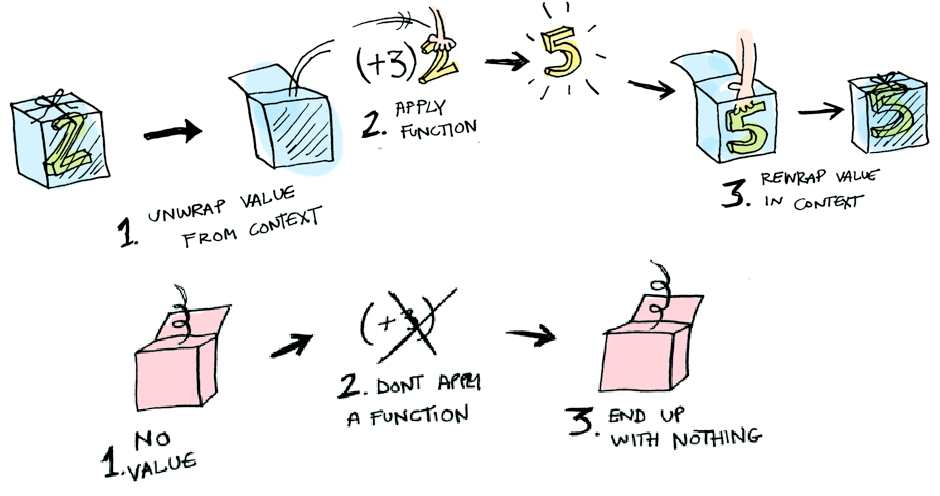
\includegraphics[scale=0.65]{images/functor}
\decoRule
\caption[functor]{Comportamento della funzione map definita da Functor[Option] \cite{FunctorsApplicativesMonads}}
\end{figure}

Oltre a fornire la propria definizione del concetto di funtore, per i tipi per cui è implementato un funtore Scalaz abilita alcuni operatori iniettati che rendono disponibile il metodo map  e altri in grado di modificare la struttura dati di partenza come as, fpair, fproduct, strengthL, strengthR, e void.

Un aspetto molto interessante è costituito dal fatto che Scalaz definisce un'istanza di funtore anche per le funzioni, che in questo caso sono viste come una mappa infinita dal dominio al codominio. Così, usando il metodo map, è possibile comporre due o più funzioni, anche se con un'anomalia non trascurabile: l'ordine è invertito rispetto alla classica composizione.

Tradizionalmente, la composizione di f e g porta ad ottenere una funzione corrispondente all'esecuzione di g seguita dall'esecuzione di f. Al contrario nei Functor di Scalaz, dato che map è un metodo iniettato in F[A], la prima funzione eseguita è f e sul suo risultato viene poi applicata g.

\lstinputlisting[caption=Definizione di Functor e semplici esempi d'uso]{code/Functor.scala}

\subsection{Apply e Applicative}

Un funtore consente di applicare una funzione ad un valore all'interno di un contesto, ma se anche la funzione fosse racchiusa in un contesto? Per consentire l'applicazione della funzione nel caso descritto Scalaz introduce Apply[F[$\_$]], un'estensione di Functor[F] che espone un metodo \textit{ap}. Si tratta di una versione potenziata di \textit{map}, poiché estrae una funzione da un contesto e successivamente applica map su un valore usando la funzione estratta. 

Inoltre Scalaz abilita gli operatori iniettati <*>, alias simbolico per il metodo \textit{ap}, *> e <*, variazioni che restituiscono solo la parte destra o sinistra.

Scalaz raffina ulteriormente il concetto espresso con Apply, attraverso la definizione del trait Applicative[F[$\_$]]. Gli applicativi, oltre ad essere istanze di Apply, introducono il metodo \textit{point} (e il suo alias \textit{pure}) che prende un valore di qualsiasi tipo e lo restituisce all'interno del contesto per cui è stato definito l'applicativo. Inoltre, Scalaz introduce il metodo \textit{point} per tutti i tipi di dati e consente così di trasformare un valore di tipo A in F[A].

\lstinputlisting[caption=Definizione di Apply e Applicative e esempi di utilizzo dell'operatore <*>]{code/Applicative.scala}

Seguendo lo stile introdotto con gli applicativi, Scalaz definisce anche una nuova notazione \textasciicircum(valore1, valore2, ...) \{ funzione \} che estrae i valori dai loro contesti e li applica ad una singola funzione (può essere utile perché consente di comportarsi come con gli applicativi senza dover inserire la funzione nel contesto). Questo nuovo stile presenta però un problema: non è in grado di gestire applicativi che accettano due parametri di tipo.

Per fornire lo stesso supporto anche a questi applicativi è stato introdotto \textit{Applicative Builder}, un'implementazione alternativa dello stile ispirato agli applicativi che usa la sintassi (valore1 |@| valore2 |@| ...) \{ funzione \}.

\lstinputlisting[caption=Alcuni semplici esempi con Applicative Style e Applicative Builder]{code/ApplicativeStyle.scala}

\subsection{Monad}

Nei funtori il valore a cui viene applicata la funzione si trova in un contesto, negli applicativi anche la funzione stessa è all'interno del contesto e, infine, le monadi sono una naturale estensione degli applicativi nata per risolvere i casi in cui il valore è nel contesto e deve essere applicata una funzione che accetta un valore normale e ritorna un valore all'interno del contesto.

A differenza degli applicativi, le monadi dovranno essere in grado di estrarre il valore dal loro contesto per poi applicare la funzione data.

\begin{figure}[th]
\centering
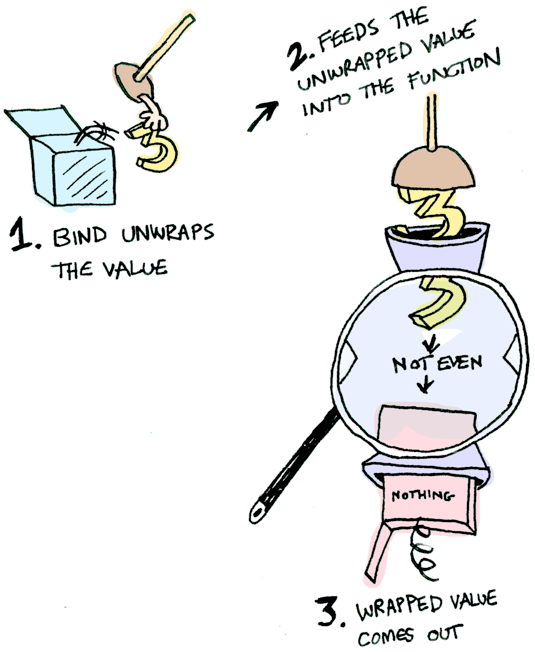
\includegraphics[scale=0.42]{images/monad}
\decoRule
\caption[monad]{Comportamento di una monade \cite{FunctorsApplicativesMonads}}
\end{figure}

Il trait Monad[F[\_]] mette a disposizione la definizione di monade di Scalaz, da cui si evince che tutte le monadi debbano essere istanze sia di Applicative[F] sia di Bind[F]. Quest'ultimo rappresenta ciò che le monadi hanno in più rispetto ai classici applicativi ed espone un metodo \textit{bind}, in grado di applicare una funzione A -> F[B] ad un valore nel suo contesto F[A]. Tutte le monadi dovranno inoltre rispettare le seguenti regole:

\begin{itemize}
\item \textit{Identità sinistra}: $\forall$ a, f, f(a) = bind(pure(a), f). Quindi se si prende un valore, si inserisce in un contesto con \textit{point} e si usa \textit{bind}, il risultato è lo stesso che si avrebbe applicando direttamente la funzione al valore.
\item \textit{Identità destra}: $\forall$ a, a = bind(a, x => pure (x)). L'elemento neutro della \textit{bind} è una funzione che restituisce il valore dato nel contesto.
\item \textit{Associatività}: $\forall$ a, f, g, bind(a, x => bind(f(x), g)) = bind(bind(a, f), g). Data una catena di applicazioni con funzioni monadiche, non importa come esse sono nidificate ma conta soltanto il loro ordine.
\end{itemize}

Come per gli altri costrutti visti, Scalaz fornisce ai tipi per cui è definita una monade il metodo \textit{bind} tramite l'operatore \textit{flatmap} e il suo alias >>=.

\lstinputlisting[caption=Definizione di Monad e dell'operatore flatMap]{code/Monad.scala}

Un aspetto da tenere in grande considerazione quando si parla di monadi è il fatto che questo tipo di astrazioni, abilitando l'operatore \textit{flatMap}, possano essere usate in una \textit{for comprehension}. Così facendo, sarà possibile concatenare in modo semplice e leggibile una serie di applicazioni di funzione.

\lstinputlisting[caption=Semplice esempio di composizione monadica senza e con l'utilizzo della for comprehension]{code/MonadFor.scala}

%----------------------------------------------------------------------------------------
%	SECTION 2
%----------------------------------------------------------------------------------------

\section{Sezione 2}

%----------------------------------------------------------------------------------------
%	SECTION 3
%----------------------------------------------------------------------------------------

\section{Sezione 3}
